\PassOptionsToPackage{quiet}{xeCJK}
\documentclass[withoutpreface,bwprint]{cumcmthesis}

\usepackage{longtable}  
\usepackage{geometry}
\geometry{left=2.5cm, right=2.5cm, top=2.5cm, bottom=2.5cm}

% 中文字号调整
\renewcommand{\rmdefault}{ptm}  % Times New Roman
\zihao{-4}  % 四号
\renewcommand{\arraystretch}{1.4}

% 表格与排版
\usepackage{tabularx}
\usepackage{booktabs}  % 三线表
\usepackage{makecell}  % \Xhline
\usepackage{diagbox}   % 斜线表头
\newcolumntype{C}{>{\centering\arraybackslash}X}
\newcolumntype{R}{>{\raggedleft\arraybackslash}X}
\newcolumntype{L}{>{\raggedright\arraybackslash}X}
\usepackage{etoolbox}
\BeforeBeginEnvironment{tabular}{\zihao{-5}}

% 数学公式
\usepackage{amsmath,amssymb}

% 文献管理
\usepackage[numbers,sort&compress]{natbib}  

% 链接、图形
\usepackage{url}
\usepackage{subcaption}  

% TikZ 绘图
\usepackage{tikz}
\usetikzlibrary{calc, arrows.meta, positioning, shapes.geometric, fit, backgrounds, decorations.text}

% 框架
\usepackage[framemethod=TikZ]{mdframed}

% 自定义颜色与命令
\definecolor{mygray}{RGB}{208,208,208}
\definecolor{mymagenta}{RGB}{226,150,116}
\newcommand*{\mytextstyle}{\sffamily\Large\bfseries\color{black!85}}

\newcommand{\arcarrow}[3]{%
   \pgfmathsetmacro{\rin}{1.7}
   \pgfmathsetmacro{\rmid}{2.2}
   \pgfmathsetmacro{\rout}{2.7}
   \pgfmathsetmacro{\astart}{#1}
   \pgfmathsetmacro{\aend}{#2}
   \pgfmathsetmacro{\atip}{5}
   \fill[mygray, very thick] (\astart+\atip:\rin)
                         arc (\astart+\atip:\aend:\rin)
      -- (\aend-\atip:\rmid)
      -- (\aend:\rout)   arc (\aend:\astart+\atip:\rout)
      -- (\astart:\rmid) -- cycle;
   \path[
      decoration = {
         text along path,
         text = {|\mytextstyle|#3},
         text align = {align = center},
         raise = -1.0ex
      },
      decorate
   ](\astart+\atip:\rmid) arc (\astart+\atip:\aend+\atip:\rmid);
}

\tikzset{
  >={Latex[width=2mm,length=2mm]},
  base/.style = {rectangle, rounded corners, draw=black,
                 minimum width=4cm, minimum height=1cm,
                 text centered, font=\sffamily},
  startstop/.style = {base, fill=red!30},
  decision/.style = {diamond, draw, text centered, inner sep=0pt,
                     minimum width=4cm, minimum height=1cm, aspect=2,
                     font=\sffamily},
  process/.style = {base, minimum width=3.5cm, fill=orange!15,
                    font=\ttfamily},
}

% 文档基本信息
\title{生产过程中的决策问题}
\tihao{}
\baominghao{}
\schoolname{}
\membera{}
\memberb{}
\memberc{}
\supervisor{}
\yearinput{}
\monthinput{}



%%%%%%%%%%%%%%%%%%%%%%%%%%%%%%%%%%%%%%%%%%%%%%%%%%%%%%%%%%%%%
%% 正文
\begin{document}

\maketitle
\thispagestyle{empty}
\begin{abstract}


本文聚焦企业电子产品生产流程中的核心决策问题,通过构建数学模型与量化分析,系统解决了抽样检测方案设计、单工序生产决策优化及多工序多零配件场景下的综合决策难题,为企业平衡成本与风险、提升运营效益提供了系统性解决方案。

\textbf{对于问题一},针对在 10\% 标称次品率下设计 95\% 与 90\% 信度下检测次数最少的抽样方案这一需求,我们基于统计假设检验理论构建模型。首先设定零假设(样本比例等于标称值)与备择假设(样本比例偏离标称值),利用中心极限定理将次品数量的分布近似为正态分布,推导样本容量计算方法。
\begin{table}[h!]
\centering
\begin{tabularx}{\textwidth}{XXXXX}
\Xhline{2pt}
\noalign{\vskip 1pt}
\toprule
置信水平 & 临界值 $Z_{\alpha/2}$ & 容忍区间 $d$ & 标称次品率 $p_0$ & 最小样本量 $n$ \\
\midrule
95\% & 1.960 & 0.02 & 0.10 & 865 \\
90\% & 1.645 & 0.02 & 0.10 & 609 \\
\bottomrule
\noalign{\vskip 1pt}
\Xhline{2pt}
\end{tabularx}
\end{table}

\textbf{对于问题二},基于六种零配件与成品参数组合,构建包含资源回收机制的多轮迭代利润模型,以最大化总利润为目标优化生产决策。模型采用\textbf{0-1 规划} 求解,考虑成品销售收益、检测成本、装配成本、调换损失及拆解后的零件循环利用价值。通过枚举法对 16 种可能策略组合进行计算。

\textbf{对于问题三},将模型推广至多道工序、多个零配件的通用场景,针对给定的 2 道工序、8 个零配件流程,构建包含半成品与零件双循环回收的利润模型。模型新增半成品检测与拆解决策,引入\textbf{遗传算法}解决多变量带来的计算复杂性。求解结果显示,最优策略为 “全零配件检测 + 全半成品检测 + 不检测成品 + 成品拆解 + 半成品 2 和 3 拆解”,此时单位利润最大(74.8344 元)。该策略通过早期检测降低次品流转风险,同时利用拆解回收高价值资源,实现了多环节成本与收益的动态平衡。

最后,本文分析了模型的优缺点:经验公式与0-1规划模型简洁高效,但存在对次品独立性假设的局限及变量增多时计算复杂度激增的问题,并提出结合成本整合优化与智能算法改进的方向,模型可推广至供应链质检、可靠性测试等多领域。

 

   \keywords{\textbf{抽样检测方案};\textbf{遗传算法};\textbf{0-1规划};\textbf{OC 曲线};\textbf{多工序生产}} 

\end{abstract}
%%%%%%%%%%%%%%%%%%%%%%%%%%%%%%%%%%%%%%%%%%%%%%%%%%%%%%%%%%%%% 

% \tableofcontents  % 目录
% \newpage

%%%%%%%%%%%%%%%%%%%%%%%%%%%%%%%%%%%%%%%%%%%%%%%%%%%%%%%%%%%%%  
\pagenumbering{arabic}
\section{问题重述}

\subsection{问题背景}
为高效利用有效资源、减少生产成本、提高运营收益,优化生产决策是每个企业经营管理中的核心环节。某企业生产电子产品需采购两种零配件,并将其装配后形成成品,且成品合格性受零配件质量影响,因此企业需通过抽样检测控制零配件次品率,并对不合格成品选择报废或拆解。生产过程中需决策是否检测零配件或成品、是否拆解不合格品,并考虑调换市场退回品的损失。对此我们需要设计抽样方案、优化生产阶段决策,并推广到多工序多零配件场景,以通过成本与风险平衡提升整体效益。


\subsection{题设数据}
\textbf{表一}给出了两种零配件和成品的次品率,以及购买单价、检测成本、市场售价等参数信息。

\textbf{表二}给出了八个零配件在两道工序中的次品率、购买单价、检测成本、拆解费用等参数信息。

\textbf{图一}给出了给出了2道工序、8个零配件的基本流程





\subsection{需要解决问题}

\textbf{问题一:}在$10\%$的标称度下,求出在$95\%$与$90\%$的信度下使检测次数尽可能少的抽样检测方案。

\textbf{问题二:}基于给定的六种情况下零配件与成品的参数,给出使利润最大化的最优生产决策方案。

\textbf{问题三:}在m道工序、n个零配件生产系统中,基于各环节的次品率、成本和售价等参数,制定最优的检测、拆解和调换决策方案,并对给定的2道工序、8个零配件给出具体决策依据和量化结果。


%%%%%%%%%%%%%%%%%%%%%%%%%%%%%%%%%%%%%%%%%%%%%%%%%%%%%%%%%%%%% 

\section{模型假设}
\textbf{假设一:}零配件的次品率相互独立,且与成品的次品率相互独立。

\textbf{假设二:}厂家每轮生产策略相同,即递归过程中零配件的次品率不变。

\textbf{假设三:}合格成品的市场售价与不合格成品的调换损失为定值,不随市场需求变化。

\textbf{假设四:}单位零配件所产生的期望利润相同。




%%%%%%%%%%%%%%%%%%%%%%%%%%%%%%%%%%%%%%%%%%%%%%%%%%%%%%%%%%%%% 

\newpage
\section{符号说明}
\begin{table}[H]
\begin{center}
 \begin{tabularx}{\textwidth}{XXX}
\Xhline{2pt}
\noalign{\vskip 1pt}
\toprule
符号    & 说明    & 单位 \\
\midrule
$n$ & 样本数 & - \\
$Z_{\alpha}$ & 临界值 & - \\
$\alpha$ & 置信度 & - \\
$p_0$ & 标称值 & - \\
$H_0$ & 零假设 & - \\
$H_1$ & 备择假设 & - \\
$X$ & 次品数量 & 个\\
$p$ & 次品率 & - \\
$d$ & 容忍区间 & - \\
$\Pi$ & 总利润期望 & 元 \\
$q$ & 合格率 & - \\
$c_{j}$ & 单位零件成本 & 元 \\
$s$ & 市场售价 & 元 \\
$x_{ij}$ & 第$i$道工序中第$j$个部件检测状态 & - \\
$d_{ij}$ & 第$i$道工序中第$j$个部件检测成本 & 个 \\
$a_{j}$ & 单位成品装配成本 & 元 \\
$t$ & 拆解成本 & 元 \\
$l$ & 调换损失 & 元 \\
$\theta $ & 回收比例 & - \\
\bottomrule
\noalign{\vskip 1pt}
\Xhline{2pt}
\end{tabularx}   
\end{center}
(其余符号详见正文)

\end{table}


%%%%%%%%%%%%%%%%%%%%%%%%%%%%%%%%%%%%%%%%%%%%%%%%%%%%%%%%%%%%% 
\newpage
\section{问题分析}
\subsection{对问题一的分析}
题目要求我们在标称值确定的情况下,设计出一种合理的抽样检测方案,使得在给定的两种不同情形下,抽样的次数最小。要使抽样的次数最小,即使得抽样的样本容量最小即可。基于此,我们根据经典检验样本容量公式,结合题目的标称值得到理想样本比例,同时根据不同情形下的置信度确定临界值,最终计算出抽样次数。
\begin{figure}[h]
   \centering
   \resizebox{0.8\linewidth}{!}{\begin{tikzpicture}[node distance=2cm and 2cm, every node/.style={fill=white}, align=center]

  % 主流程节点
  \node (start) [startstop] {经典样本检测容量公式};
  \node (p2) [process, left=of start] {置信度临界值};
  \node (p1) [process, above  =of p2] {样本比例};
  \node (p3) [process, below  =of p2] {容忍区间};
  \node (p4) [process, above right=of start] {情形一样本容量};
  \node (p5) [process, below right=of start] {情形二样本容量};
  \begin{pgfonlayer}{background}
    \node[draw=blue,dashed, thick, inner sep=12pt, fit=(p1) (p3)] {};
  \end{pgfonlayer}
  
  \begin{pgfonlayer}{background}
    \node[draw=red, dashed, thick, inner sep=12pt, fit =(p4)(p5)] {};
  \end{pgfonlayer}
  % 分类文字单独放
  \node(text) [below=0.2cm of p3,text=blue] {\textbf{公式系数}};
  \node[below=0.2cm of p5,text=red] {\textbf{抽样次数}};
    \draw[<-,dashed] (start) |- node[midway]{标称值}(p1);
   \draw[<-,dashed] (start) -- (p2);
   \draw[<-,dashed] (start) |- node[midway]{经验值}(p3);
   \draw[->] (start) --++(2.25,0) --node[midway] {置信度为95\%}(p4);
   \draw[->] (start) --++(2.25,0) -- node[midway] {置信度为90\%}(p5);

  
\end{tikzpicture}}
   \caption{第一问流程图}
   \label{fig:one}
\end{figure}
\subsection{对问题二的分析}
题目要求我们设计出一种最优的生产决策方案,使得在给定的六种情况下,利润最大化。我们首先对各工序之间的关系,绘制了如下流程图:
\begin{figure}[h]
   \centering
   \resizebox{0.9\linewidth}{!}{\begin{tikzpicture}[node distance=2cm and 2cm, every node/.style={fill=white}, align=center]

  % 主流程节点
  \node (start) [startstop] {经典样本检测容量公式};
  \node (p2) [process, left=of start] {置信度临界值};
  \node (p1) [process, above  =of p2] {样本比例};
  \node (p3) [process, below  =of p2] {容忍区间};
  \node (p4) [process, above right=of start] {情形一样本容量};
  \node (p5) [process, below right=of start] {情形二样本容量};
  \begin{pgfonlayer}{background}
    \node[draw=blue,dashed, thick, inner sep=12pt, fit=(p1) (p3)] {};
  \end{pgfonlayer}
  
  \begin{pgfonlayer}{background}
    \node[draw=red, dashed, thick, inner sep=12pt, fit =(p4)(p5)] {};
  \end{pgfonlayer}
  % 分类文字单独放
  \node(text) [below=0.2cm of p3,text=blue] {\textbf{公式系数}};
  \node[below=0.2cm of p5,text=red] {\textbf{抽样次数}};
    \draw[<-,dashed] (start) |- node[midway]{标称值}(p1);
   \draw[<-,dashed] (start) -- (p2);
   \draw[<-,dashed] (start) |- node[midway]{经验值}(p3);
   \draw[->] (start) --++(2.25,0) --node[midway] {置信度为95\%}(p4);
   \draw[->] (start) --++(2.25,0) -- node[midway] {置信度为90\%}(p5);

  
\end{tikzpicture}}
   \caption{各工序关系流程图}
   \label{fig:one}
\end{figure}

为定量刻画检测与拆解策略在多轮装配过程中的利润演化情况,本文建立了一个包含资源回收机制的多轮迭代模型。假设在初始轮次中系统仅使用原始投入的零部件,装配所得成品经由检测决定是否进入市场,不合格成品可选择拆解,回收所得零部件将进入下一轮生产。模型在每一轮中动态更新原材料结构,重构装配过程中的次品率与资源使用情况,并据此计算当轮利润。

在利润计算方面,每一轮均考虑成品销售收益、检测成本、装配成本、调换成本与拆解成本。成品利润受检测策略影响,若跳过检测,次品流入市场将引致一定的损失;若实施检测,则可避免售后损失但需承担检测成本。同时,拆解策略决定回收零部件的数量和质量,进而影响下一轮的装配结构与合格率,利润也由此产生间接影响。

最终,系统的长期收益由所有轮次的利润叠加构成,其中每一轮利润会乘以回收带来的资源贡献程度。通过控制迭代次数,直到收益收敛,我们能够更全面地评估不同检测与拆解策略的长期经济效益,为企业在资源循环利用背景下的决策优化提供可靠依据,得到利润最大化的生产决策方案。
\begin{figure}[h]
   \centering
   \resizebox{0.5\linewidth}{!}{\begin{tikzpicture}[node distance=2cm and 2cm, every node/.style={fill=white}, align=center]
\def\layersep{4cm}

\tikzstyle{goal node}=[circle,fill=red!50,minimum size=18pt,inner sep=0pt]
\tikzstyle{criteria node}=[circle,fill=blue!50,minimum size=18pt,inner sep=0pt]
\tikzstyle{option node}=[circle,fill=green!50,minimum size=18pt,inner sep=0pt]
\tikzstyle{annot} = [text width=4em, text centered]

% 目标层
\node[goal node] (G) at (0, 0) {};
\node[below= 0.3cm of G] {期望利润};

% 准则层(成本构成3个方面)
\node[criteria node] (C1) at (\layersep, 2) {};
\node[below= 0.3cm of C1] {收入};

\node[criteria node] (C2) at (\layersep, -2) {};
\node[below= 0.3cm of C2] {成本};



% 目标->准则
\foreach \x in {1,2}
    \draw[->] (G) -- (C\x);

% 方案层(可以细化各成本细节)
\node[option node] (O0) at (2*\layersep, 3) {};
\node[below= 0.3cm of O0] {期望收入};

\node[option node] (O1) at (2*\layersep, 1) {};
\node[below= 0.5cm of O1] {零件检测成本};

\node[option node] (O2) at (2*\layersep, -1) {};
\node[below= 0.3cm of O2] {成品检测成本};

\node[option node] (O3) at (2*\layersep, -3) {};
\node[below= 0.3cm of O3] {次品拆解成本};   

\node[option node] (O4) at (2*\layersep, -5) {};
\node[below= 0.3cm of O4] {次品调换损失};


% 准则->方案(示意连接)
\draw[->] (C1) -- (O0);
\foreach \x in {1,2,3,4}
    \draw[->] (C2) -- (O\x);

% 层名注释
\node[annot] at (0, 4) {一级结构};
\node[annot] at (\layersep, 4) {二级结构};
\node[annot] at (2*\layersep, 4) {三级结构};


\end{tikzpicture}
}
   \caption{利润结构图}
   \label{fig:one}
\end{figure}
\subsection{对问题三的分析}
题目要求我们设计出一种最优的检测、拆解和调换决策方案,并对给定的2道工序、8个零配件给出具体决策依据和量化结果。我们基于第二问的模型,对利润结构进行适当的重构,引入半成品工序所导致一系列成本。同时由于半成品工序的存在,我们需要对循环利润进行适当调整,即在零件回收利润的基础上,引入了半成品回收利润。最后将得到目标函数利用遗传算法进行优化,得到利润最大化的生产决策方案。

%%%%%%%%%%%%%%%%%%%%%%%%%%%%%%%%%%%%%%%%%%%%%%%%%%%%%%%%%%%%% 
\newpage
\newpage
\section{问题一的模型的建立和求解}
\subsection{模型建立}
\subsubsection{假设框架}
根据题设条件,我们构建了如下假设框架:
\begin{itemize}
   \item 零假设$H_0$:样本比例$p$等于标称值$p_0$
   \item 备择假设$H_1$:对于拒收情形,样本比例$p$大于标称值$p_0$;对于接受情形,样本比例$p$小于标称值$p_0$。
\end{itemize}
\subsubsection{样本容量公式}
假设从总体中抽取容量为$n$的样本,记其中的次品个数为随机变量$X$,显然该变量服从二项分布$X \sim Bin(n,p)$。
其中$p$为样本比例。根据中心极限定理,当$n$足够大时,$X$可以近似服从正态分布,即\begin{equation}
X\sim N(np,np(1-p))
\end{equation}
进一步的,我们可确定样本中的次品率的统计量$\hat{p}$近似服从正态分布,即
\begin{equation}
\hat{p}\sim N(p,\frac{p(1-p)}{n})
\end{equation}
由上式我们可推导出经典样本检测容量公式
\begin{equation}
n=\frac{Z^2_{\alpha}p(1-p)}{d^2}
\end{equation}
其中$Z_{\alpha}$为置信区间在标准正态分布中的临界值,$\alpha$为置信度,$d$为容忍区间,一般取经验值。

\subsection{模型求解}
将题设条件代入上式,同时,我们取容忍区间为0.02,最终求得结果如下表
\begin{table}[h!]
\centering
\caption{不同置信水平下的样本量计算($d = 0.02$, $p_0 = 0.10$)}
\begin{tabularx}{\textwidth}{XXXXX}
\Xhline{2pt}
\noalign{\vskip 1pt}
\toprule
置信水平 & 临界值 $Z_{\alpha/2}$ & 容忍区间 $d$ & 标称次品率 $p_0$ & 最小样本量 $n$ \\
\midrule
95\% & 1.960 & 0.02 & 0.10 & 865 \\
90\% & 1.645 & 0.02 & 0.10 & 609 \\
\bottomrule
\noalign{\vskip 1pt}
\Xhline{2pt}
\end{tabularx}
\end{table}

由表可知,在95\%置信水平下,临界值$Z_{\alpha/2}=1.960$,容忍区间$d=0.02$,标称次品率$p_0=0.10$,最小样本量$n=865$。在90\%置信水平下,临界值$Z_{\alpha/2}=1.645$,容忍区间$d=0.02$,标称次品率$p_0=0.10$,最小样本量$n=609$。

\subsection{结果分析}
上述结果表明,若零件总数远大于最小样本量时,无论样本容量为何值时,样本容量取结果值时能取到满足题设条件与统计约束上的最优值。

为进一步验证得到的样本容量的合理性,本文拟采用OC曲线对结果进行可视化分析,OC曲线反映了在不同实际不合格率$p$下,产品被接受的概率$P_{\text{accept}}$。

通过计算,并绘制了如下的OC曲线:

\begin{figure}[h!]
\centering
\subcaptionbox{样本空间为865的OC曲线\label{fig:双图a}}
{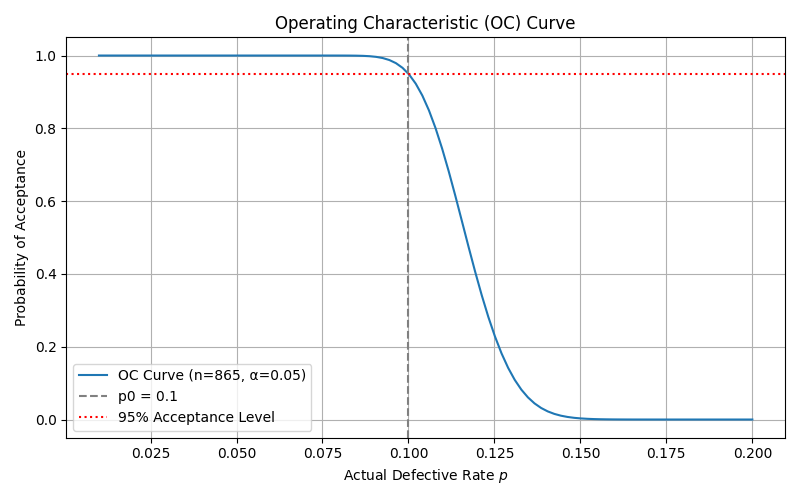
\includegraphics[width=.49\textwidth]{figure/OC_curve_1.png}}
\subcaptionbox{样本空间为609的OC曲线\label{fig:双图b}}
{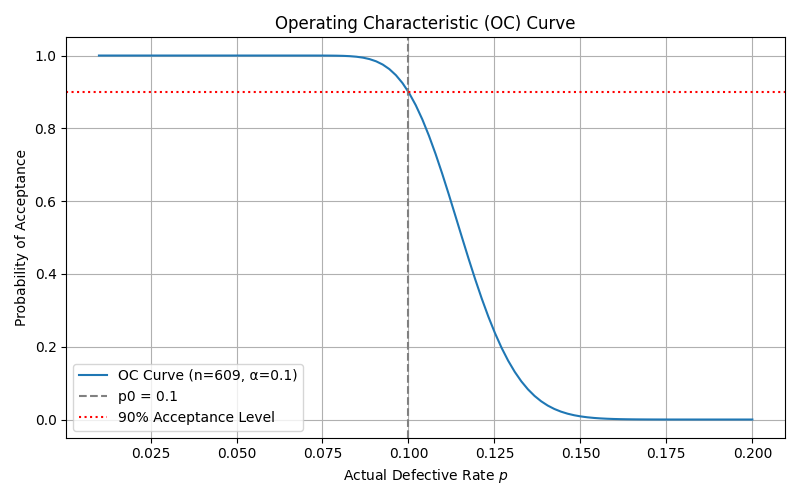
\includegraphics[width=.49\textwidth]{figure/OC_curve_2.png}}
\caption{双图}\label{fig:双图}
\end{figure} 

利用OC曲线可以直观地观察在不同实际不合格率下当前抽样计划的接受概率。从图\ref{fig:双图a}中不难发现,当实际不合格率接近标称值$p_0=0.10$时,接受概率约为95\%,与设定置信水平一致;特别地,我们注意到,随着实际不合格率上升,接受概率陡然下降,说明该检验方案对不合格产品的敏感性较高,即对不合格产品的识别能力较强。

同时,对于质量较好的批次,该方案也能保持较高的接受概率,体现了良好的灵敏度和平衡性。我们从图\ref{fig:双图b}也能得到类似的结论。

此外,根据OC曲线我们还能得出,该种抽样方案下对不合格品的最大容忍数$n_{\text{max}}$,即若发现样本容量中不合格数大于该数值,则拒收,其算式为
\begin{equation}
   n_{\text{max}}=\frac{Z_{\alpha/2}^2p_0(1-p_0)}{d^2}
\end{equation}

对于情形一而言,$n_{\text{max}}=103$,即若抽样容量中不合格数大于103,则拒收。对于情形二而言,$n_{\text{max}}=74$,即若抽样容量大于74,则拒收。

%%%%%%%%%%%%%%%%%%%%%%%%%%%%%%%%%%%%%%%%%%%%%%%%%%%%%%%%%%%%% 
\section{问题二的模型的建立和求解}
\subsection{模型建立}
\subsubsection{决策变量设立}
针对本问题中装配企业对零配件与成品的检测及拆解决策,我们从全局最优的角度出发,希望最大化企业的期望利润。由于每道工序(如零件检测、成品检测、成品拆解)均为可选动作,决策结果具有离散性,故本问题可建模为一个0-1整数规划问题。

故我们引入如下决策变量:
\begin{itemize}
   \item $x_{ij}$:第$i$道工序中第$j$个零件的\textbf{检测状态},$x_{ij}=1$表示检测通过,$x_{ij}=0$表示检测不通过。特别地,$x_f$代表成品检测状态。
   \item $d_{ij}$:第$i$道工序中第$j$个零件的\textbf{检测成本},$d_{ij}$为非负实数,特别地,$d_f$代表成品检测成本。
   \item $a_{ij}$:第$j$个零件的单位成品\textbf{固定成本},即固定成本为零件装配成本或购买成本。$a_{j}$为非负实数。特别地,$a_f$代表成品固定成本。
   \item $t$:\textbf{总拆解成本},$t$为非负实数。
   \item $l$:\textbf{总调换损失},$l$为非负实数。
   \item $\theta_{ij}$:第$i$道工序中第$j$个零件\textbf{回收比例},$\theta$为实数。
   \item $z_{ij}$:从成品往后开始的第$i$道工序的第$j$个成品(或半成品)的\textbf{拆解状态},$z_{i}=1$表示该零件已拆解,$z_{i}=0$表示该零件未拆解。
   \item $p_{ij}$:第$i$道工序中第$j$个零件的\textbf{次品率},$p_{ij}$为实数。
   \item $q_{ij}$:第$i$道工序中第$j$个零件的\textbf{合格率},$q_{ij}=1-p_{ij}$。
   \item $k_{ij}$:第$i$道工序中第$j$个零件的\textbf{实际比例},$k_{ij}$为非负实数。特别地,$k_f$代表成品实际比例。
   \item $s$:\textbf{市场售价},$s$为非负实数。
\end{itemize}

其中每一组决策 $(x_{11}, x_{12}, ..., x_f,... ,z_{21}, z_1)$ 对应一种检测-拆解策略。
\subsubsection{目标函数构建}
由于不合格成品可被拆解,拆解出的零件可循环使用,投入到下一轮生产中时会产生对应的利润,本文称其为:“利润积累”效应。我们定义 $\pi_0$ 为第一轮循环的单位利润,$\theta$ 为每轮可回收再利用的零件比例,显然的,对于第$i$轮的利润,它等于第本轮收益乘上回收比例$\theta$,即
\begin{equation}
\pi_i=(P_i-C_i)\theta^n
\end{equation}
对于总利润而言,它等于每一轮的利润求和,则总利润的期望为:
\begin{equation}
\pi_{total}=\sum_{n=0}^{\infty}\pi_i=\pi_0+\sum_{n=1}^{\infty}(P_i-C_i)\theta^n,\quad 0<\theta<1
\end{equation}
因此,我们最后的目标函数即为:
\begin{equation}
\max\{\pi_{total}\}
\end{equation}
\subsubsection{第一轮利润的构建}
第一轮利润 $\pi_0$ 可视为初始收益减去初始成本,即
\begin{equation}
\pi_0=P_0-C_0
\end{equation}
对于初始收益而言,其数值为市场售价、成品合格率、成品实际比例三者之积,即
\begin{equation}
P_0= s q_f k_f
\end{equation}
而对于初始成本,其数值为固定成本、检测成本、拆解成本、调换损失之和,对于本问,考虑仅有一道工序、两个零件的情况,我们由如下公式计算:
\begin{equation}
C_0=\sum_{j=1}^2 (a_{1j}+x_{1j}d_{1j})+k_f (a_f+ x_fd_f + z_1t(1-q_f)+(1-x_f)(1-q_f)l)
\end{equation}
需要注意的是,$q_f$由如下算式确定:
\begin{equation}
q_f=(1-p_f)(1-(1-x_{11})p_1)(1-(1-x_{12})p_2)
\end{equation}
而$k_f$由如下算式确定:
\begin{equation}
k_f=\frac{(1-x_{11}p_1)+(1-x_{12}p_2)}{2}
\end{equation}
\subsubsection{迭代利润的构建}
以某一轮的利润$\pi_m$为例,其构成与第一轮类似,区别在于零件的成本与次品率的计算,以及回收系数的引入。

首先对于零件的成本而言,由于零件的来源为前一轮成品的拆解,故我们可以忽略其购买成本,即第一道工序中的固定成本$a_{1j}$。

对于零件的次品率,由于零件的来源为前一轮成品的拆解,由于拆解的成品必为次品,次品成品中至少含有一个次品零件,故该轮中的次品率实际为,在已知两个零件中至少含有一个次品零件与次品率(实际为上一轮的次品率)的情况下,任选一个是次品的概率,即为条件概率,易得其算式为:
\begin{equation}
p_{ij}^{(n)}=\frac{p_{ij}^{(n-1)}}{1-(1-p_{ij}^{(n-1)})^2}
\end{equation}

于是我们便有第$m$轮的收益,即
\begin{equation}
P_m=s q_f^{(m)} k_f^{(m)}
\end{equation}
而对应的成本则为:
\begin{equation}
C_m=\sum_{j=1}^2 x_{1j}d_{1j}+k_f^{(m)} (a_f+ x_fd_f + z_1t(1-q_f^{(m)})+(1-x_f)(1-q_f^{(m)})l)
\end{equation}

现在我们来确定回收系数,回收系数即从第$m-1$轮的成品中回收零件的比例,它等于第$m-1$轮的次品率、第$m-1$轮的成品实际比例、第$m-1$轮的回收系数之积,同时他还受拆解状态制约,由此我们最终有:
\begin{equation}
\theta_m=z_1(1-q_f^{(m-1)})k_f^{(m-1)}\theta_{m-1}
\end{equation}
于是,第$m$轮的利润可由如下公式计算:
\begin{equation}
\pi_m=(P_m-C_m)\theta_m
\end{equation}

最终迭代的总利润为:
\begin{equation}
\pi_{total}=\pi_0+\sum_{m=1}^{\infty}\pi_m
\end{equation}
\subsubsection{模型求解}
考虑问题二中,0-1变量仅有四个,故总情况为$2^4=16$种,即使考虑有六种不同的情形,最可能数也仅为96种,故可以采用枚举法求解。

代入表中数据,最终得到如下最优解,见表\ref{tab:最优策略}
\begin{table}[H]
\centering
\begin{tabularx}{\textwidth}{cXXXXX}
\Xhline{2pt}
\noalign{\vskip 1pt}
\toprule
情况编号 & 利润/元 & 零件1检测 & 零件2检测 & 成品检测 & 拆解 \\
\midrule
1 & 13.4047 & 是 & 是 & 否 & 是 \\
2 & 4.1750  & 是 & 是 & 否 & 是 \\
3 & 11.1390 & 是 & 是 & 否 & 是 \\
4 & 6.9998  & 是 & 是 & 是 & 是 \\
5 & 11.2487 & 否 & 是 & 是 & 是 \\
6 & 18.5867 & 否 & 否 & 否 & 否 \\
\bottomrule
\noalign{\vskip 1pt}
\Xhline{2pt}
\end{tabularx}
\caption{各情形最优策略及对应单位利润}
\label{tab:最优策略}
\end{table}
\subsection{结果分析}
通过对比可以发现,最大利润出现在情形6(18.5867元),该情况下次品率整体最低,企业选择完全不检测也不拆解,以节省各项成本,并凭借较高成品合格率实现最大化收益。相反,利润最小值出现在情形2(4.175元),该参数设定下次品率较高,且尽管执行全检测策略并启用拆解,仍难以弥补由质量波动带来的成本损耗,导致整体收益受限。

值得注意的是,情形3与情形4仅在“成品检测”上有所差异,前者选择跳过成品检测以降低成本,而后者引入成品检测以规避售后损失,二者单位利润分别为11.1390元与6.9998元,提示当拆解费用较低但调换损失较大时,是否检测成品对利润影响较显著。情形5的策略表明,在零件1质量稳定、但检测成本偏高时,放弃该零件检测反而有利于提升整体收益

为更直观展示各情形利润水平与策略分布关系,绘制如下柱状图
\begin{figure}[H]
\centering
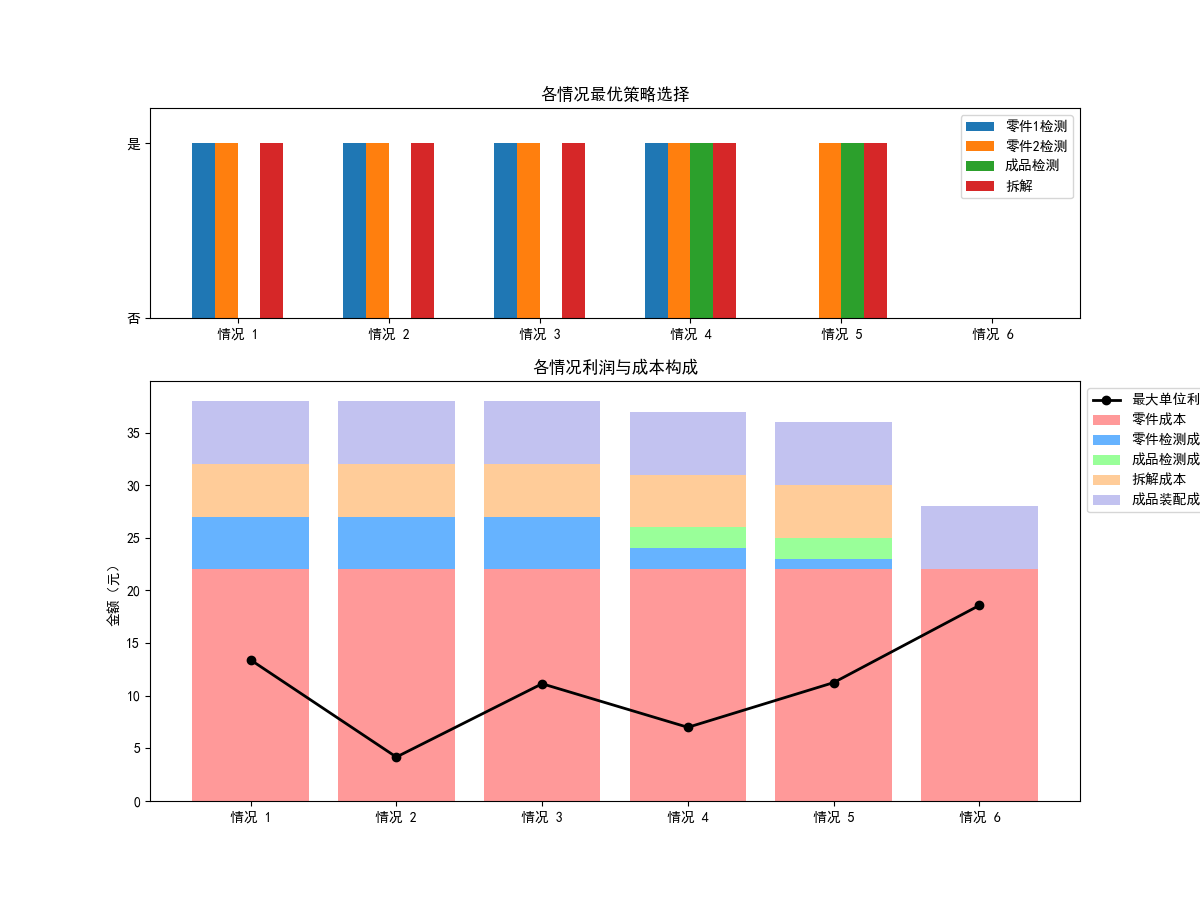
\includegraphics[width=\textwidth]{figure/fuck.png}
\caption{各情形利润与策略分布}
\end{figure}

明显的,由于情形6的成本较低,故其即使全部不检测也可获得较高收益。
%%%%%%%%%%%%%%%%%%%%%%%%%%%%%%%%%%%%%%%%%%%%%%%%%%%%%%%%%%%%% 
\section{问题三的模型的建立和求解}
\subsection{模型建立}
参照问题二的模型建立,问题三的模型建立与问题二相同,主要区别在于每轮循环的收益由半成品收益与零件收益两部分组成,即:
\begin{equation}
\pi_i={\pi_{half}}_i+{\pi_{componet}}_i
\end{equation}
其中,${\pi_{half}}_i$为第$i$轮半成品收益,${\pi_{componet}}_i$为第$i$轮零件收益。

当然,我们在此还是先给出第一轮的收益计算公式:
\begin{equation}
\pi_0=P_0-C_0
\end{equation}
对于初始收益而言,其数值为市场售价、成品合格率、成品实际比例三者之积,即
\begin{equation}
P_0= s q_f k_f
\end{equation}
而对于初始成本,其数值为固定成本、检测成本、拆解成本、调换损失之和,对于本问,考虑仅有一道工序、两个零件的情况,我们由如下公式计算:
\begin{equation}
C_0=\sum_{j=1}^8(a_{1j}+x_{1j}d_{1j})+\sum_{j=1}^{3} k_{1j}(a_{2j}+ x_{2j}d_{2j}+z_{2j}(1-q_{2j})t_{2j}) + k_f(z_1t_1(1-q_f)+(1-x_f)(1-q_f)l)
\end{equation}
需要注意的是,$q_f$由如下算式确定:
\begin{equation}
q_f=q_{21}q_{22}q_{23}(1-p_f)
\end{equation}
对于任意的下级$q_{ij}$都有类似确定方式,在此不再赘述。
而$k_f$由如下算式确定:
\begin{equation}
k_f=\frac{(1-x_{21}p_{21})k_{11}q_{11}q_{12}q_{13}+(1-x_{22}p_{22})k_{12}q_{14}q_{15}q_{16}+(1-x_{23}p_{23})k_{13}q_{17}q_{18}}{3}
\end{equation}
对于任意的下级$k_{ij}$都有类似确定方式,在此不再赘述。

接下来我们对某一轮的收益进行计算,假设第$m$轮的收益为:
\begin{equation}
\pi_m={\pi_{half}}_m+{\pi_{componet}}_m
\end{equation}
其中,${\pi_{half}}_m$为第$m$轮半成品收益,${\pi_{componet}}_m$为第$m$轮零件收益。

对于半成品收益而言,其数值为:
\begin{equation}
{P_{half}}_m=s q_f^{(m)} k_f^{(m)}
\end{equation}

半成品回收后不存在装配成本,故其成本可写作
\begin{equation}
C_{half}^{(m)}=\sum_{j=1}^{3} (a_{2j}+ x_{2j}d_{2j}+z_{2j}(1-q_{2j}^{(m)})t_{2j}) + k_f^{(m)}(z_1t_1(1-q_f^{(m)})+(1-x_f)(1-q_f^{(m)})l)
\end{equation}
对于零件收益而言,其数值为:
\begin{equation}
{P_{component}}_m=s q_{fc}^{(m)} k_{fc}^{(m)}
\end{equation}

零件回收后不存在购买成本,故其成本可写作
\begin{equation}
C_{component}^{(m)}=\sum_{j=1}^8 (x_{1j}d_{1j})+\sum_{j=1}^{3} k_{1j}(a_{2j}+ x_{2j}d_{2j}+z_{2j}(1-q_{c2j}^{(m)})t_{2j}) +k_f^{(m)}(z_1t_1(1-q_{fc}^{(m)})+(1-x_f)(1-q_{fc}^{(m)})l)
\end{equation}

其中$q_{fc}^{m}$与$k_{fc}^{m}$及其相关衍生公式的确定方法同问题二,不再赘述。

最后,来确定回收系数,由于存在两种不同的回收利润,故回收系数也分为两种,分别为$\theta_{half}$与$\theta_{component}$,其计算公式如下:
\begin{equation}
\theta_{half}^{(m)}=z_1(1-q_f^{(m-1)})*k_f^{(m-1)}+z_1(1-q_{fc}^{(m-1)})*k_{fc}^{(m-1)}\theta_{beta}^{(m-1)}\theta_{half}^{(m-1)}
\end{equation}
\begin{equation}
\theta_{component}^{(m)}=\frac{3z_{21}(1-q_{21}^{m-1})+3z_{22}(1-q_{22}^{m-1})+2z_{23}(1-q_{23}^{m-1})}{8}
\end{equation}

最后我们可以确定第$m$轮的收益,即:
\begin{equation}  
\pi_m=({P_{half}}_{m}-C_{half}^{(m)})\theta_{half}^{(m)}+({P_{component}}_{m}-C_{component}^{(m)})\theta_{component}^{(m)}
\end{equation}

总收益对上式进行求和即可
\subsection{模型求解}
由于决策变量变为了16个,模型求解情况指数级增长,求解起来较为困难,故我们采用遗传算法,在每轮迭代种,得出最稳健的解,并将其作为下一轮种群的初始种群。最终输出我们需要的决策集合,即使得利润最大的策略。

将题中数据代入模型,最终求得最优策略如下:


\begin{longtable}{p{0.5\textwidth}p{0.4\textwidth}}
\caption{最佳检测与拆解策略下的各项决策取值(单位利润最大值:74.8344)} \\
\toprule
\textbf{决策项} & \textbf{取值} \\
\midrule
\endfirsthead

\multicolumn{2}{l}{\textit{续表:最佳检测与拆解策略下的各项决策取值}} \\
\toprule
\textbf{决策项} & \textbf{取值} \\
\midrule
\endhead

\bottomrule
\endfoot

零配件1       & 是 \\
零配件2       & 是 \\
零配件3       & 是 \\
零配件4       & 是 \\
零配件5       & 是 \\
零配件6       & 是 \\
零配件7       & 是 \\
零配件8       & 是 \\
半成品1       & 是 \\
半成品2       & 是 \\
半成品3       & 是 \\
成品          & 否 \\
成品拆解      & 是 \\
半成品1拆解   & 否 \\
半成品2拆解   & 是 \\
半成品3拆解   & 是 \\
\end{longtable}

见表可得,最大利润为74.8344元。
\subsection{结果分析}
本研究建立了一个多级装配系统的检测与拆解策略优化模型,涵盖零配件、半成品及成品的检测和拆解决策,目标是最大化单位产品的期望利润。在充分考虑各类次品率、检测成本、装配费用、成品售价、拆解费用与调换损失等因素的基础上,我们穷举了所有$2^{16}$种可能策略组合,并计算每种方案对应的利润水平。结果表明,最优策略是在所有零配件与半成品阶段均进行检测,放弃成品检测,但保留对成品及部分半成品的拆解选项,最终单位利润达到最大值74.8344元。

从策略组合分析来看,检测确实带来成本增加,但在装配早期就发现并隔离次品,有效提高了最终成品的合格率,减少了调换损失,使得整体收益上升。同时,成品检测成本较高,且不能回收资源,放弃成品检测、改用拆解方式回收半成品和零配件,不仅节省了成本,也提高了资源利用率。最终策略正是检测与拆解之间实现平衡的最优解。

\begin{figure}[H]
\centering
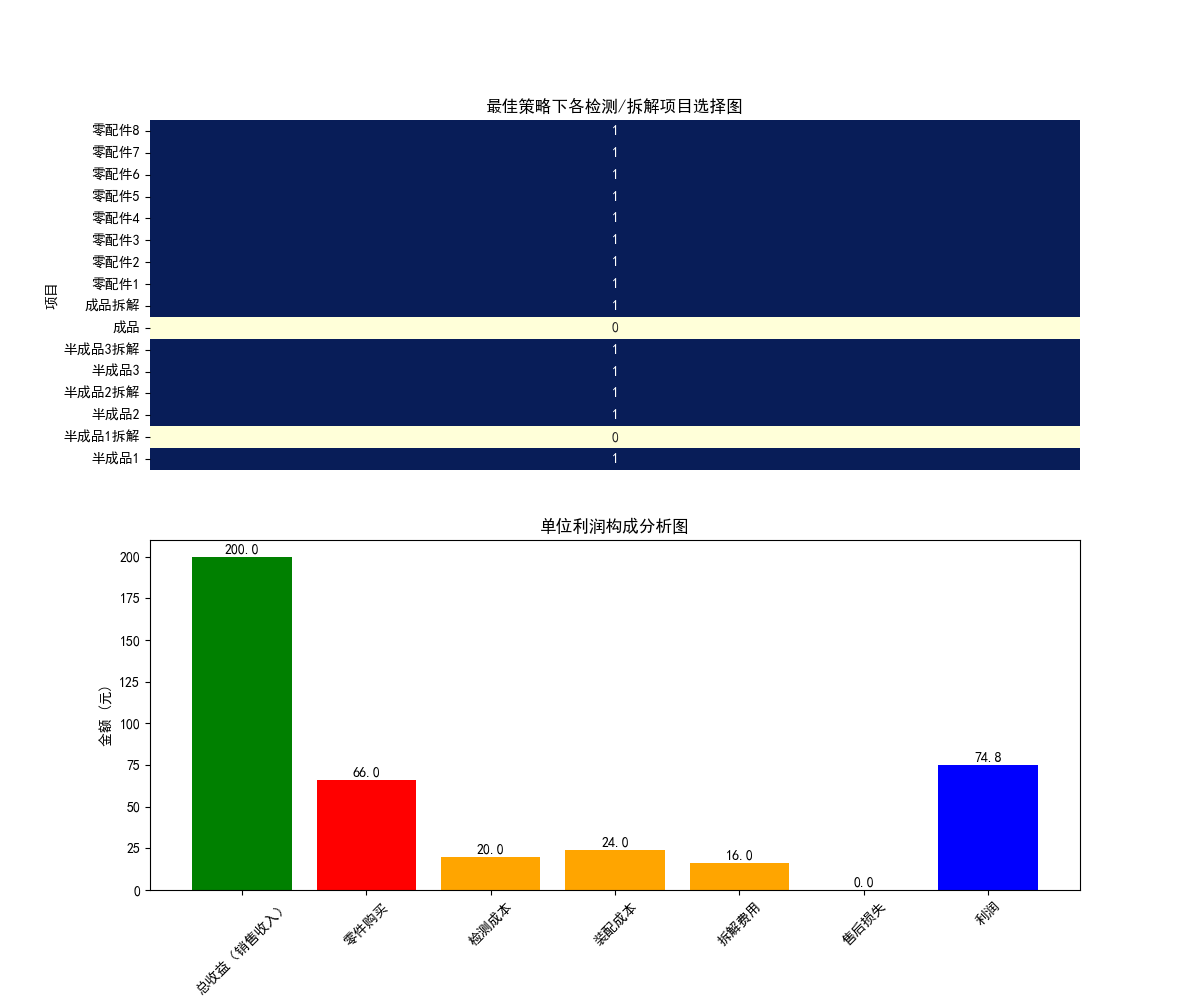
\includegraphics[width=\textwidth]{figure/final.png}
\caption{各情形利润与策略分布}
\end{figure}
从结果图上可以看出,不同策略下的合格率、成本和利润三者之间呈现显著的权衡关系。最佳策略在检测投入和资源回收之间取得了协调,从而最大程度地提升了系统整体的经济效益,为复杂制造流程中的策略制定提供了量化依据和优化路径。
\section{模型的评价}

\subsection{模型的优点}
\begin{itemize}[itemindent=2em]
\item 优点1:经验样本容量公式计算简便,无需复杂统计工具,并且很好的控制了两类错误,即生产方风险和使用方风险。在信度要求变化时,公式能灵活调整抽样方案,实现了动态调整。

\item 优点2:0-1规划整合复杂逻辑约束,简要精准的描述了“是否”类二元决策问题,简化了模型,适用于多阶段决策。

\end{itemize}

\subsection{模型的缺点}
\begin{itemize}[itemindent=2em]
\item 缺点1:问题一假设样本中的次品出现是独立且概率恒定的,但实际生产中,次品可能集中在某些批次,此时抽样结果会低估真实风险。

\item 缺点2:0-1规划的计算复杂度高,变量增多时求解时间指数级增长,增大计算难度。


\end{itemize}
%%%%%%%%%%%%%%%%%%%%%%%%%%%%%%%%%%%%%%%%%%%%%%%%%%%%%%%%%%%%%

\section{模型的改进与推广}

\subsection{改进}
\begin{itemize}[itemindent=2em]
   \item 改进1:问题一可进行成本整合优化:将公式嵌入决策树或线性规划,同时优化样本量、检测成本、拆解费用等。
   \item 改进2:
\end{itemize}


\subsection{推广}
\begin{itemize}[itemindent=2em]
    \item 推广1:经验样本容量公式可推广到供应商来料检验、电子产品可靠性测试与寿命评估、市场质量反馈与售后分析等实际问题。
   \item 推广2:0-1规划可推广到投资组合优化、电路设计、广告投放、网络与路径优化等所有二元决策类问题。
\end{itemize}
\newpage
%%%%%%%%%%%%%%%%%%%%%%%%%%%%%%%%%%%%%%%%%%%%%%%%%%%%%%%%%%%%%
%% 参考文献
\nocite{*}
\bibliographystyle{gbt7714-numerical}  % 引用格式
\bibliography{ref.bib}  % bib源

\newpage
%%%%%%%%%%%%%%%%%%%%%%%%%%%%%%%%%%%%%%%%%%%%%%%%%%%%%%%%%%%%%
%% 附录
\begin{appendices}
\section{文件列表}
\begin{table}[H]
\centering
\begin{tabularx}{\textwidth}{LL}
\toprule
文件名   & 功能描述 \\
\midrule
 exercise\_1.py & 问题一程序代码 \\
 exercise\_2.py & 问题二程序代码 \\
 exercise\_3.py & 问题三程序代码 \\

\bottomrule
\end{tabularx}
\label{tab:文件列表}
\end{table}

\section{代码}
\noindent 
 exercise\_1.py
\lstinputlisting[language=python]{code/exercise_1.py}
exercise\_2.py
\lstinputlisting[language=python]{code/exercise_2.py}
exercise\_3.py
 \lstinputlisting[language=python]{code/exercise_3.py}


\end{appendices}
\end{document}


%%%%%双图模板%%%%%%
% \begin{figure}
% \centering
% \subcaptionbox{炉温曲线示意图\label{fig:双图a}}
% {\includegraphics[width=.4\textwidth]{炉温曲线示意图.png}}
% \subcaptionbox{问题1炉温曲线\label{fig:双图b}}
% {\includegraphics[width=.4\textwidth]{问题1炉温曲线.png}}
% \caption{双图}\label{fig:双图}
% \end{figure} 
%%%%%双图模板%%%%%%